\section{Technische Spezifikationen}\label{TechnischeSpezifikationen}
\subsection{Systemübersicht}\label{Systemuebersicht}
Die folgenden Kapitel bieten einen Überblick über die Hauptkomponenten der Maschine, deren Funktion und ihre technischen Möglichkeiten.
\subsubsection{Steuerungseinheit}
Die gesamte Technik wird mithilfe von zwei Netzteilen, ein 12-Volt- und ein 24-Volt-Netzteil, mit Strom versorgt. An das 12 Volt Gerät ist wiederum ein Spannungswandler, welcher die passende Spannung von 5 Volt an den Raspberry Pi (Raspberry Pi 4 Model B) weiterleitet. Dieser fungiert als zentrale Steuerungseinheit. In ihm steckt eine SD Karte, auf der die Software gespeichert ist, welche die grafische Oberfläche erzeugt, sowie die Steuerungslogik, mit welcher die anderen Komponenten angesteuert werden. Eine dieser anderen Komponenten ist das Acht-Kanal-Relais, über welches die Pumpen einzeln oder zusammen angesteuert und auch hin und zurück pumpen können. Weiterhin sind an dem Pi die Driver der Stepper-Motoren und der Linearmotor selber angeschlossen.\newline

Im Bild \ref{unten} sind alle Komponenten der Steuerungseinheit zu sehen.
\subsubsection{Linearantrieb}
Im vorherigen Kapitel wurde ein Linearmotor erwähnt, dieser ist fest an dem Linearantrieb angebracht und sorgt dafür das der Spritzkopf in X-Richtung, entlang der großen Gewindestange, bewegt werden kann. Der Linearantrieb fährt mit einer Geschwindigkeit von \textit{hier die Geschwindigkeit noch angeben}, und erreicht die gesetzten Positionen auf den Zehntelmilimeter genau. \newline

\begin{figure}[H] % r = rechts, l = links
    \centering
    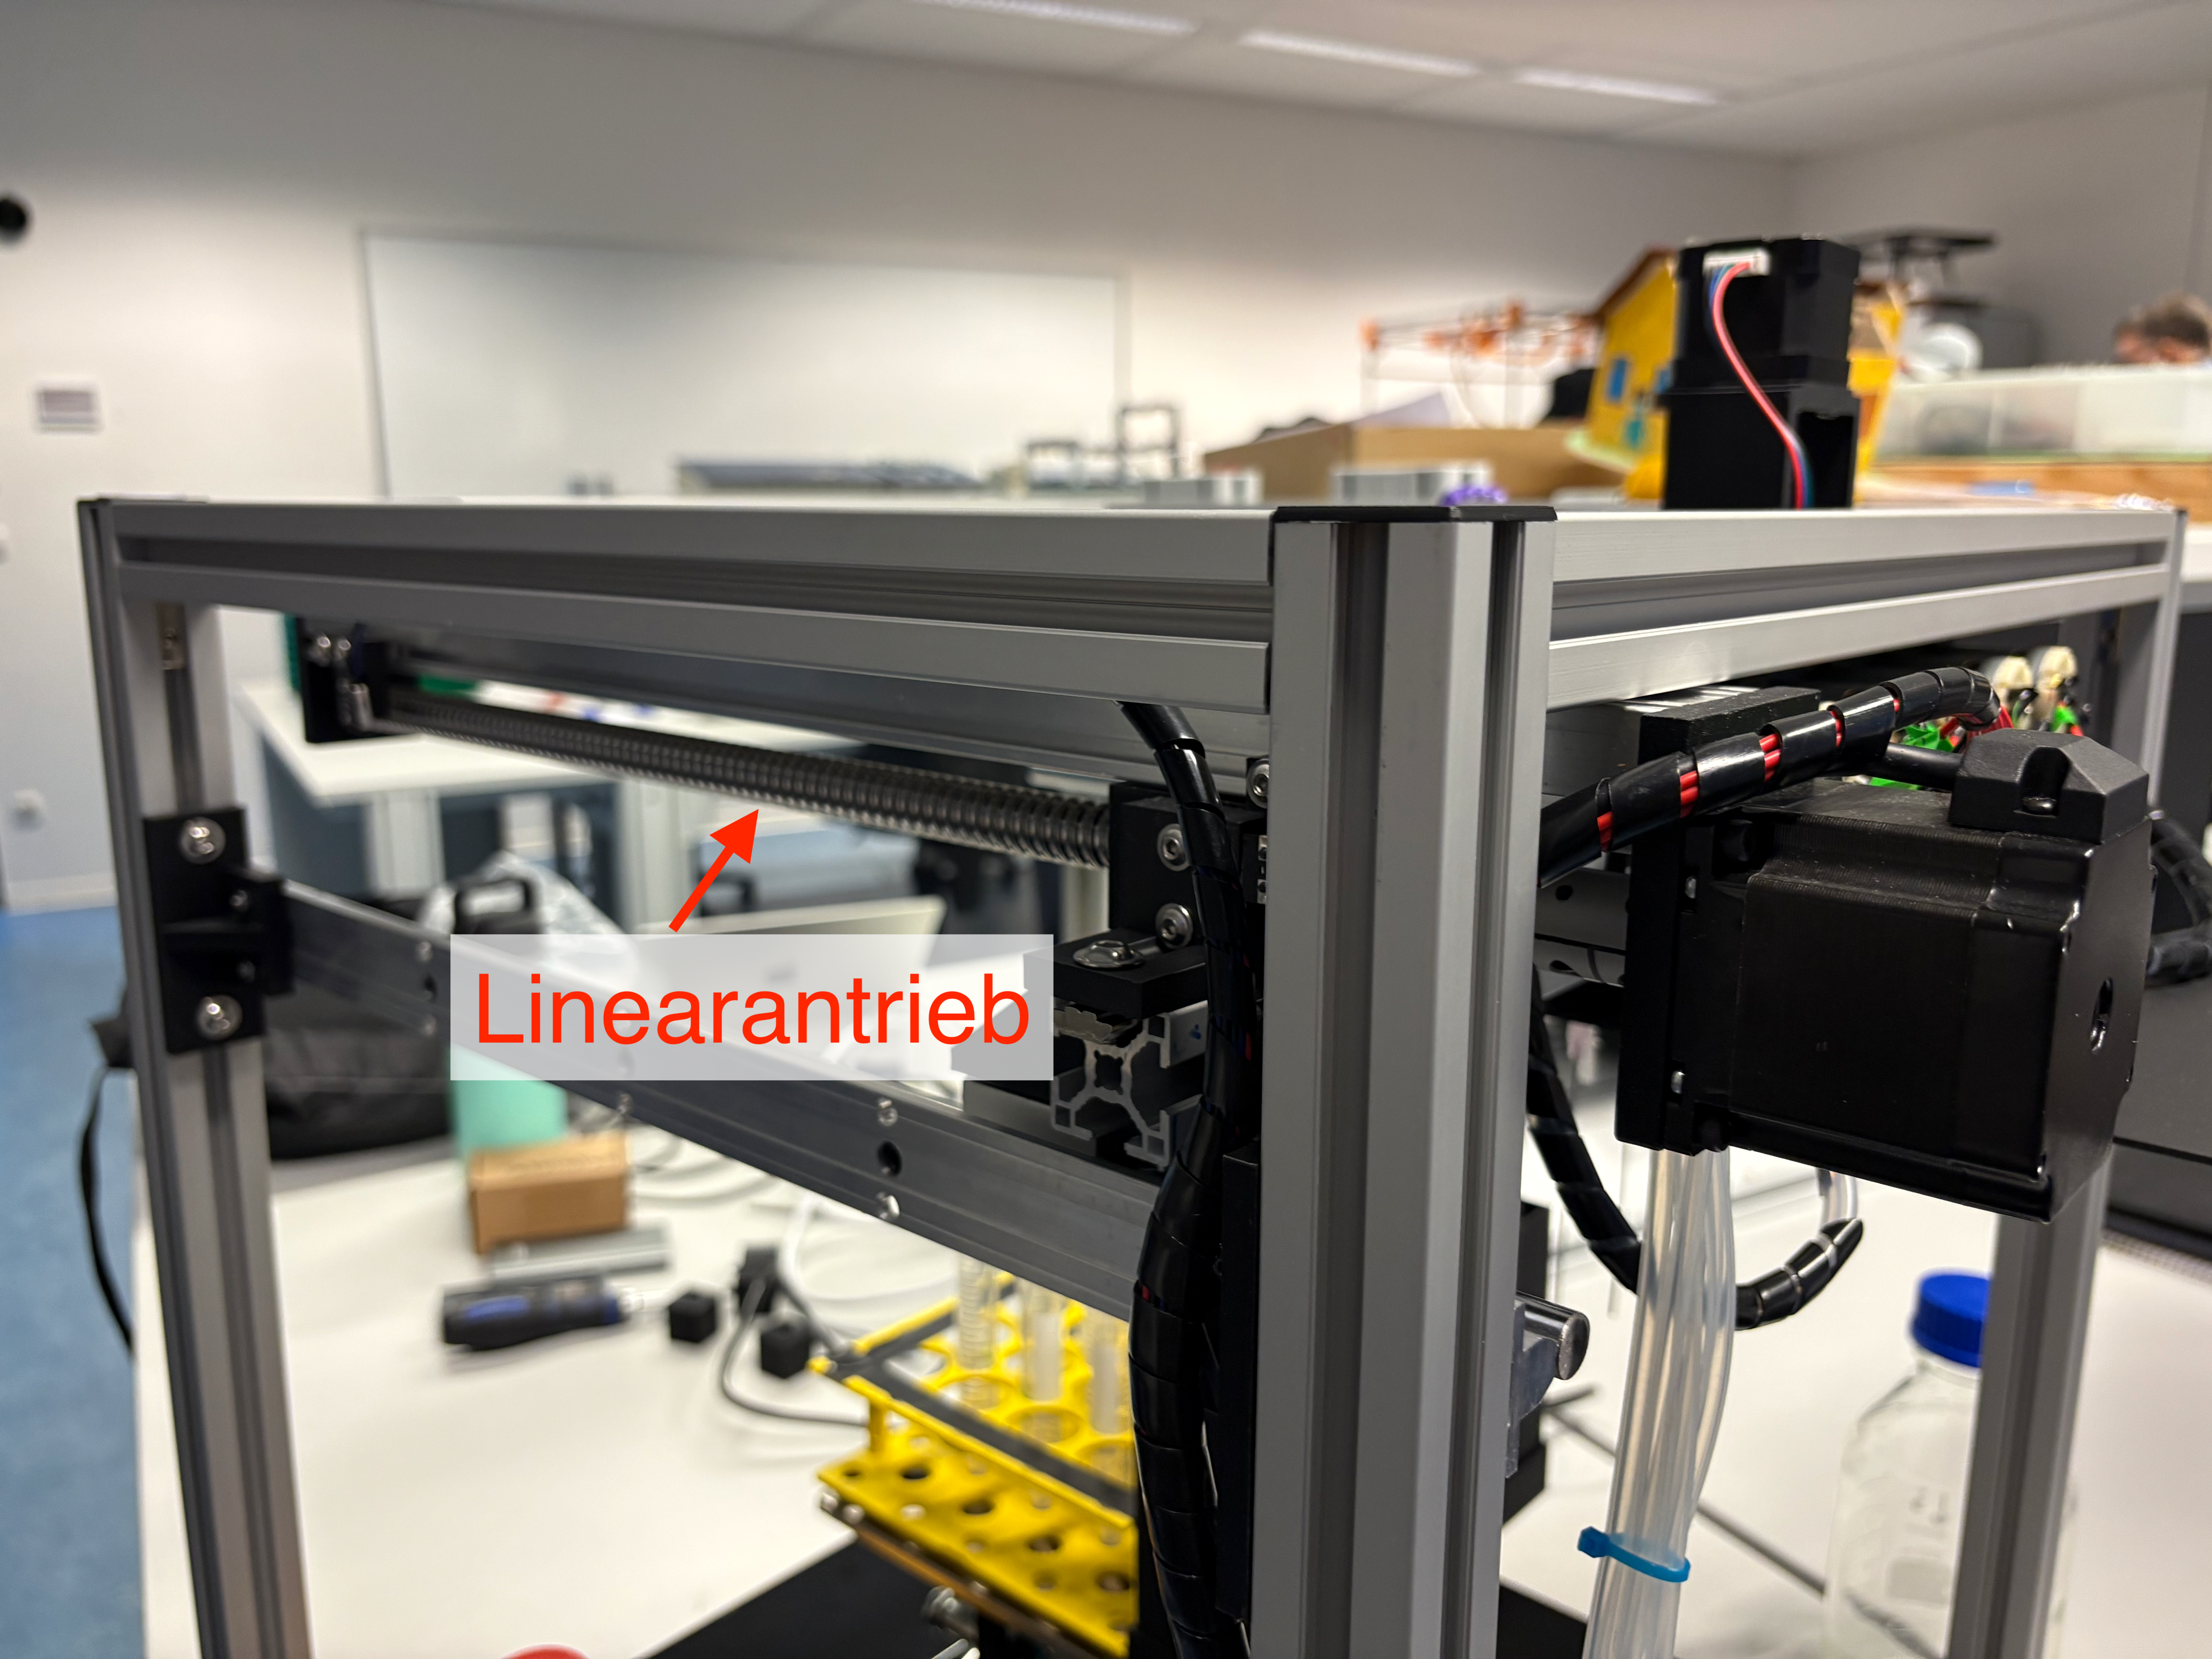
\includegraphics[width=0.8\textwidth]{images/Linear.png}
    \caption{Linearantrieb des Probenverdünners}
    \label{linear}
\end{figure}
\newpage
\subsubsection{Pumpen}
Insgesamt werden in dieser Maschine fünf Pumpen verwendet, die das Verdünnungsmittel mit einem maximalen Fehler von 0,5 \% auf 10 ml aufziehen. Diese Pumpen werden durch das Relai-Modul gesteuert, sodass jede Pumpe einzeln angesteuert werden kann. Dies ermöglicht uns einzelne Spalten zu deaktivieren. Außerdem können wir dadurch minimale Abweichungen pro Pumpe ausgleichen. Im Betrieb wird jeweils in Schritten von 1ml gepumpt. Alle Pumpen starten dabei zeitgleich, aber enden zeitversetzt, sodass jede Pumpe genau 1ml gepumpt hat und danach alle wieder synchronisiert sind. An jeder Pumpe sind 2 Schläuche befestigt. Einer davon ist fest verbunden mit dem Spritzenkopf, der jeweils andere (also 5 verbleibende Schläuche) müssen vor Start des Programms in die Schottflasche gelegt werden. Diese muss zu jeder Zeit einen Mindestfüllstand von 50ml haben. \newline

\begin{figure}[H] % r = rechts, l = links
    \centering
    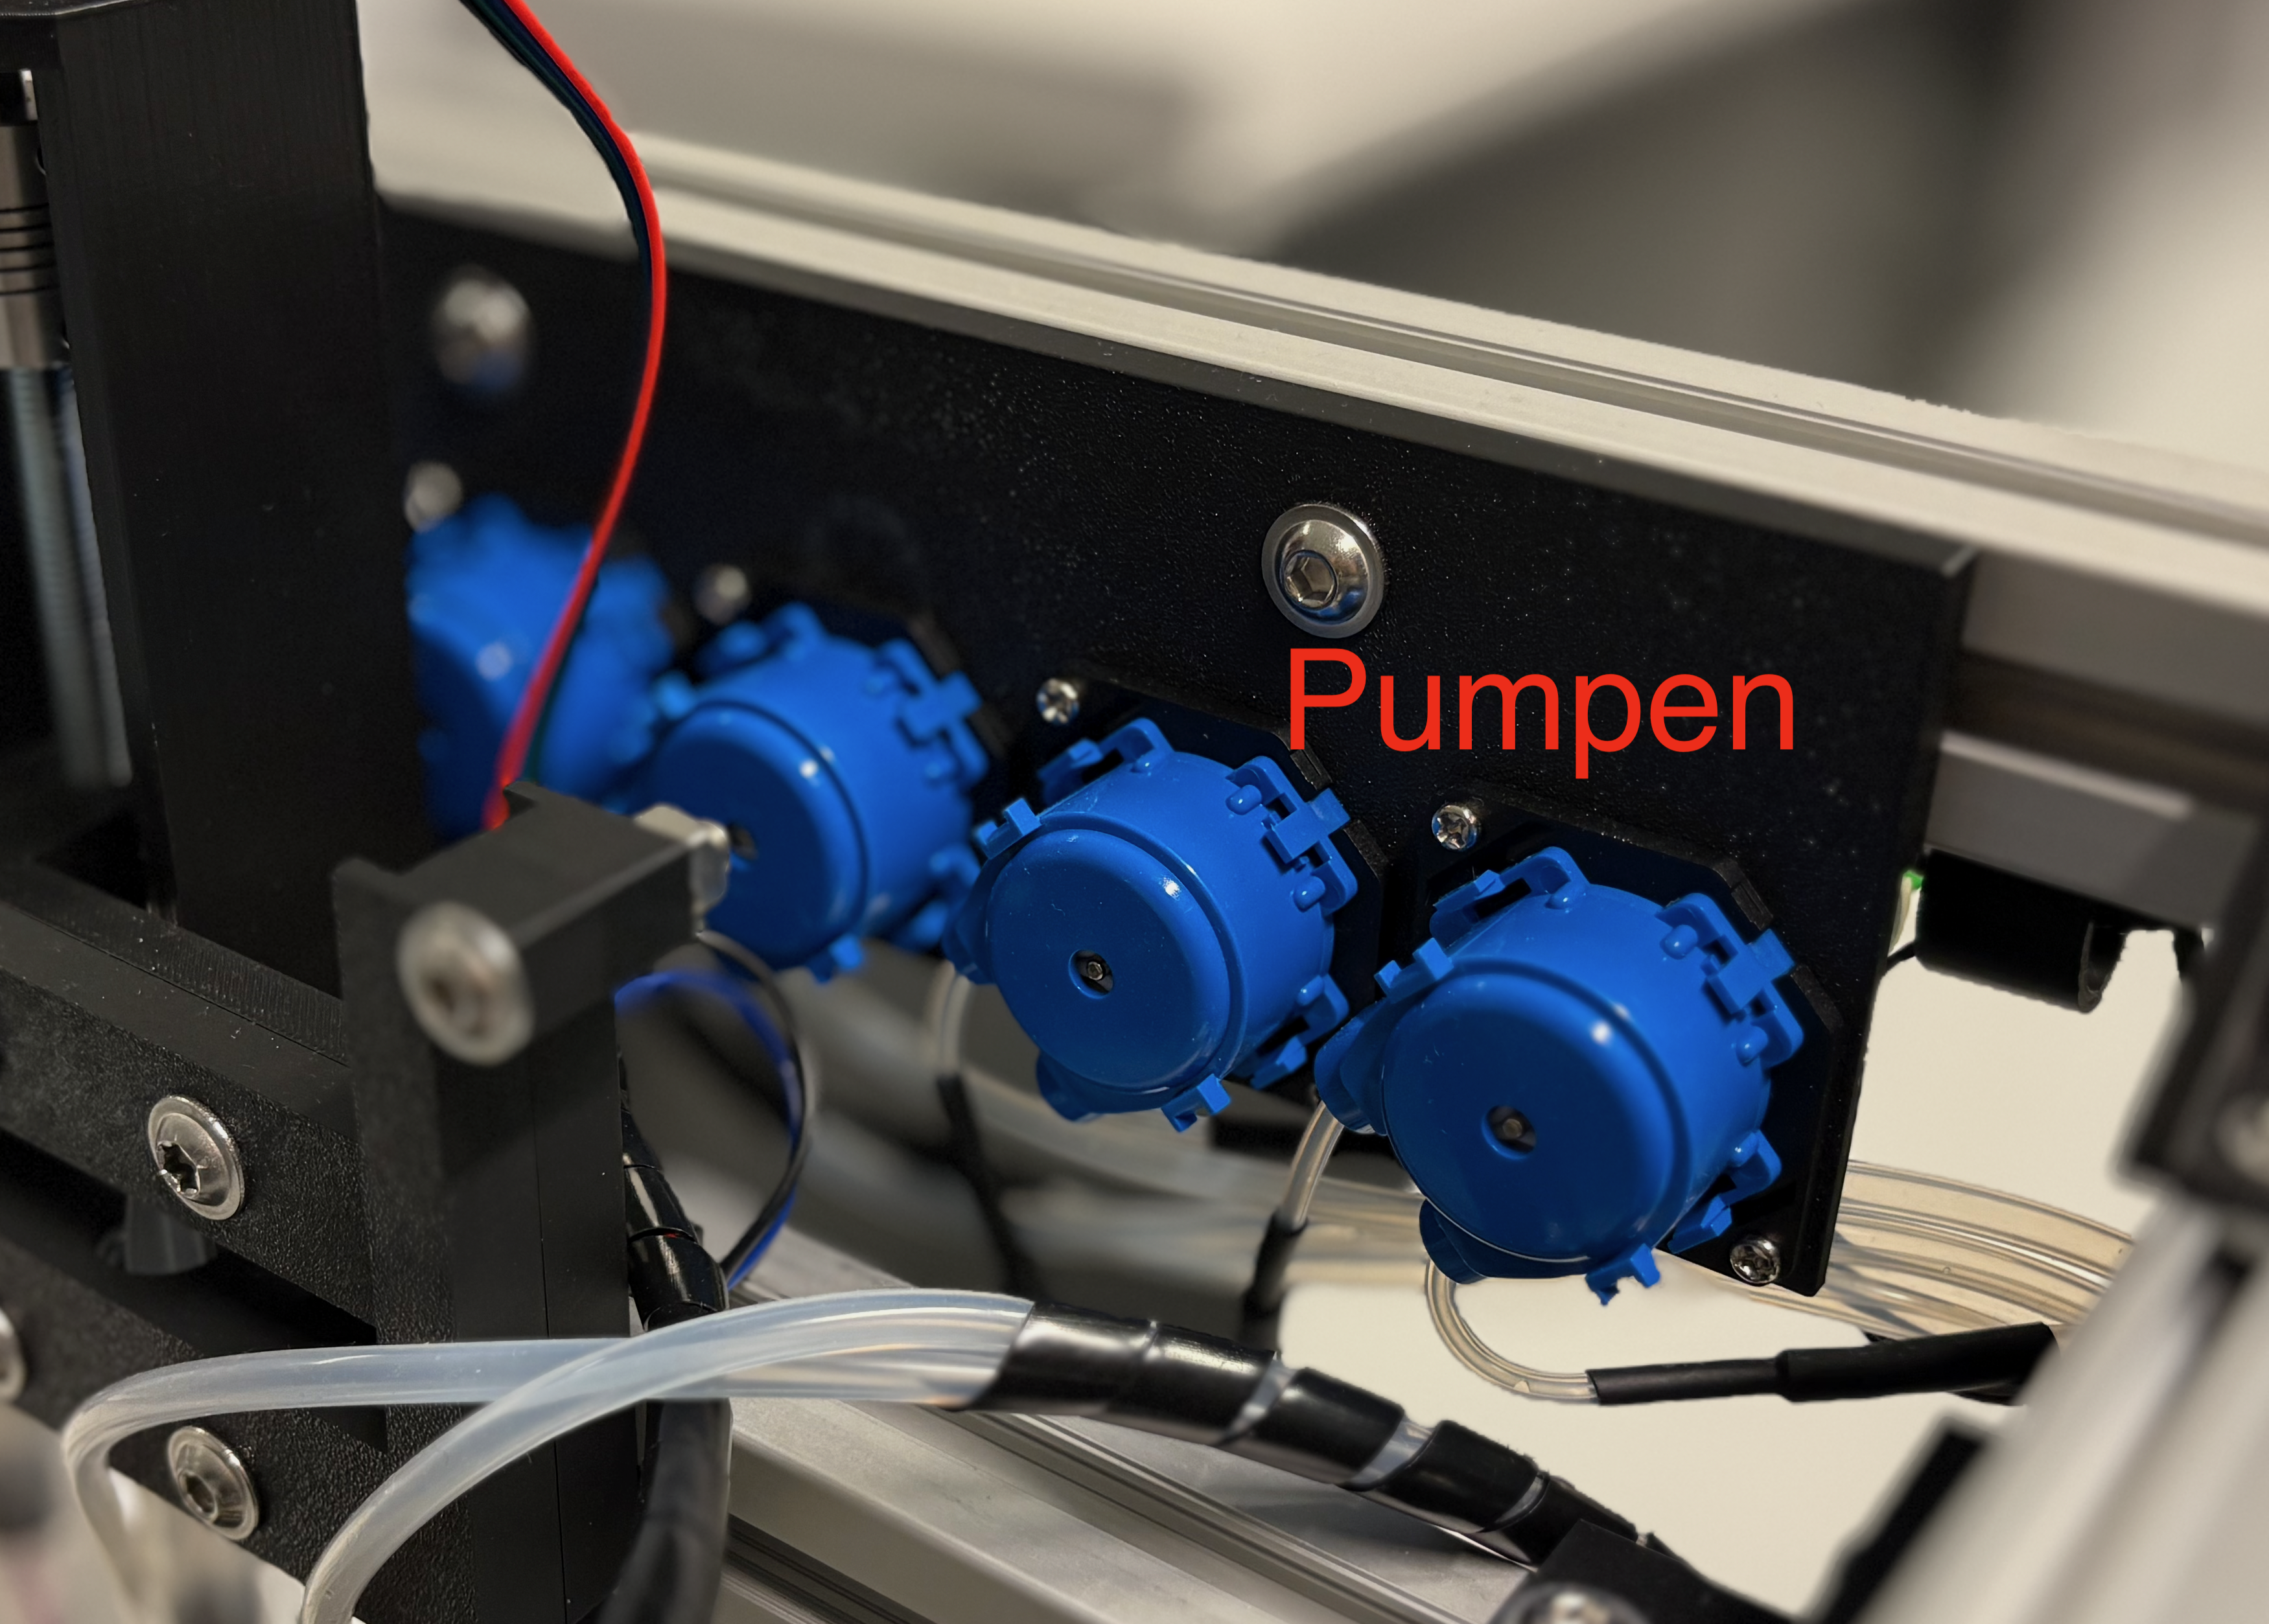
\includegraphics[width=0.8\textwidth]{images/pumpen.png}
    \caption{Pumpen des Probenverdünners}
    \label{pumpen}
\end{figure}
\newpage
\subsubsection{Spritzenkopf}
Der Spritzenkopf ist an einem Aluprofil befestigt, welches zwischen zwei Linearführung befestigt ist. Er wird von dem Linearantrieb betrieben. An ihm sind dazu noch fünf Spritzen und Schläuche montiert, welche die Falcontubes befüllen. Die Spritzen werden über einen Steppermotor und einem 3D-gedrucktem Konstrukt gleichmäßg und gleichzeitig aufgezogen, sodass fünf Proben oder weniger gleichzeitig befüllt oder entnommen werden können. Die Spritzen arbeiten mit einem maximalen Fehler von 3\% auf 1 ml. Zuletzt ist an dem Spritzkopf noch eine Platte befestigt, welche am Ende einer Verdünnung die Falcontubes bedecken kann.\newline

\begin{figure}[H] % r = rechts, l = links
    \centering
    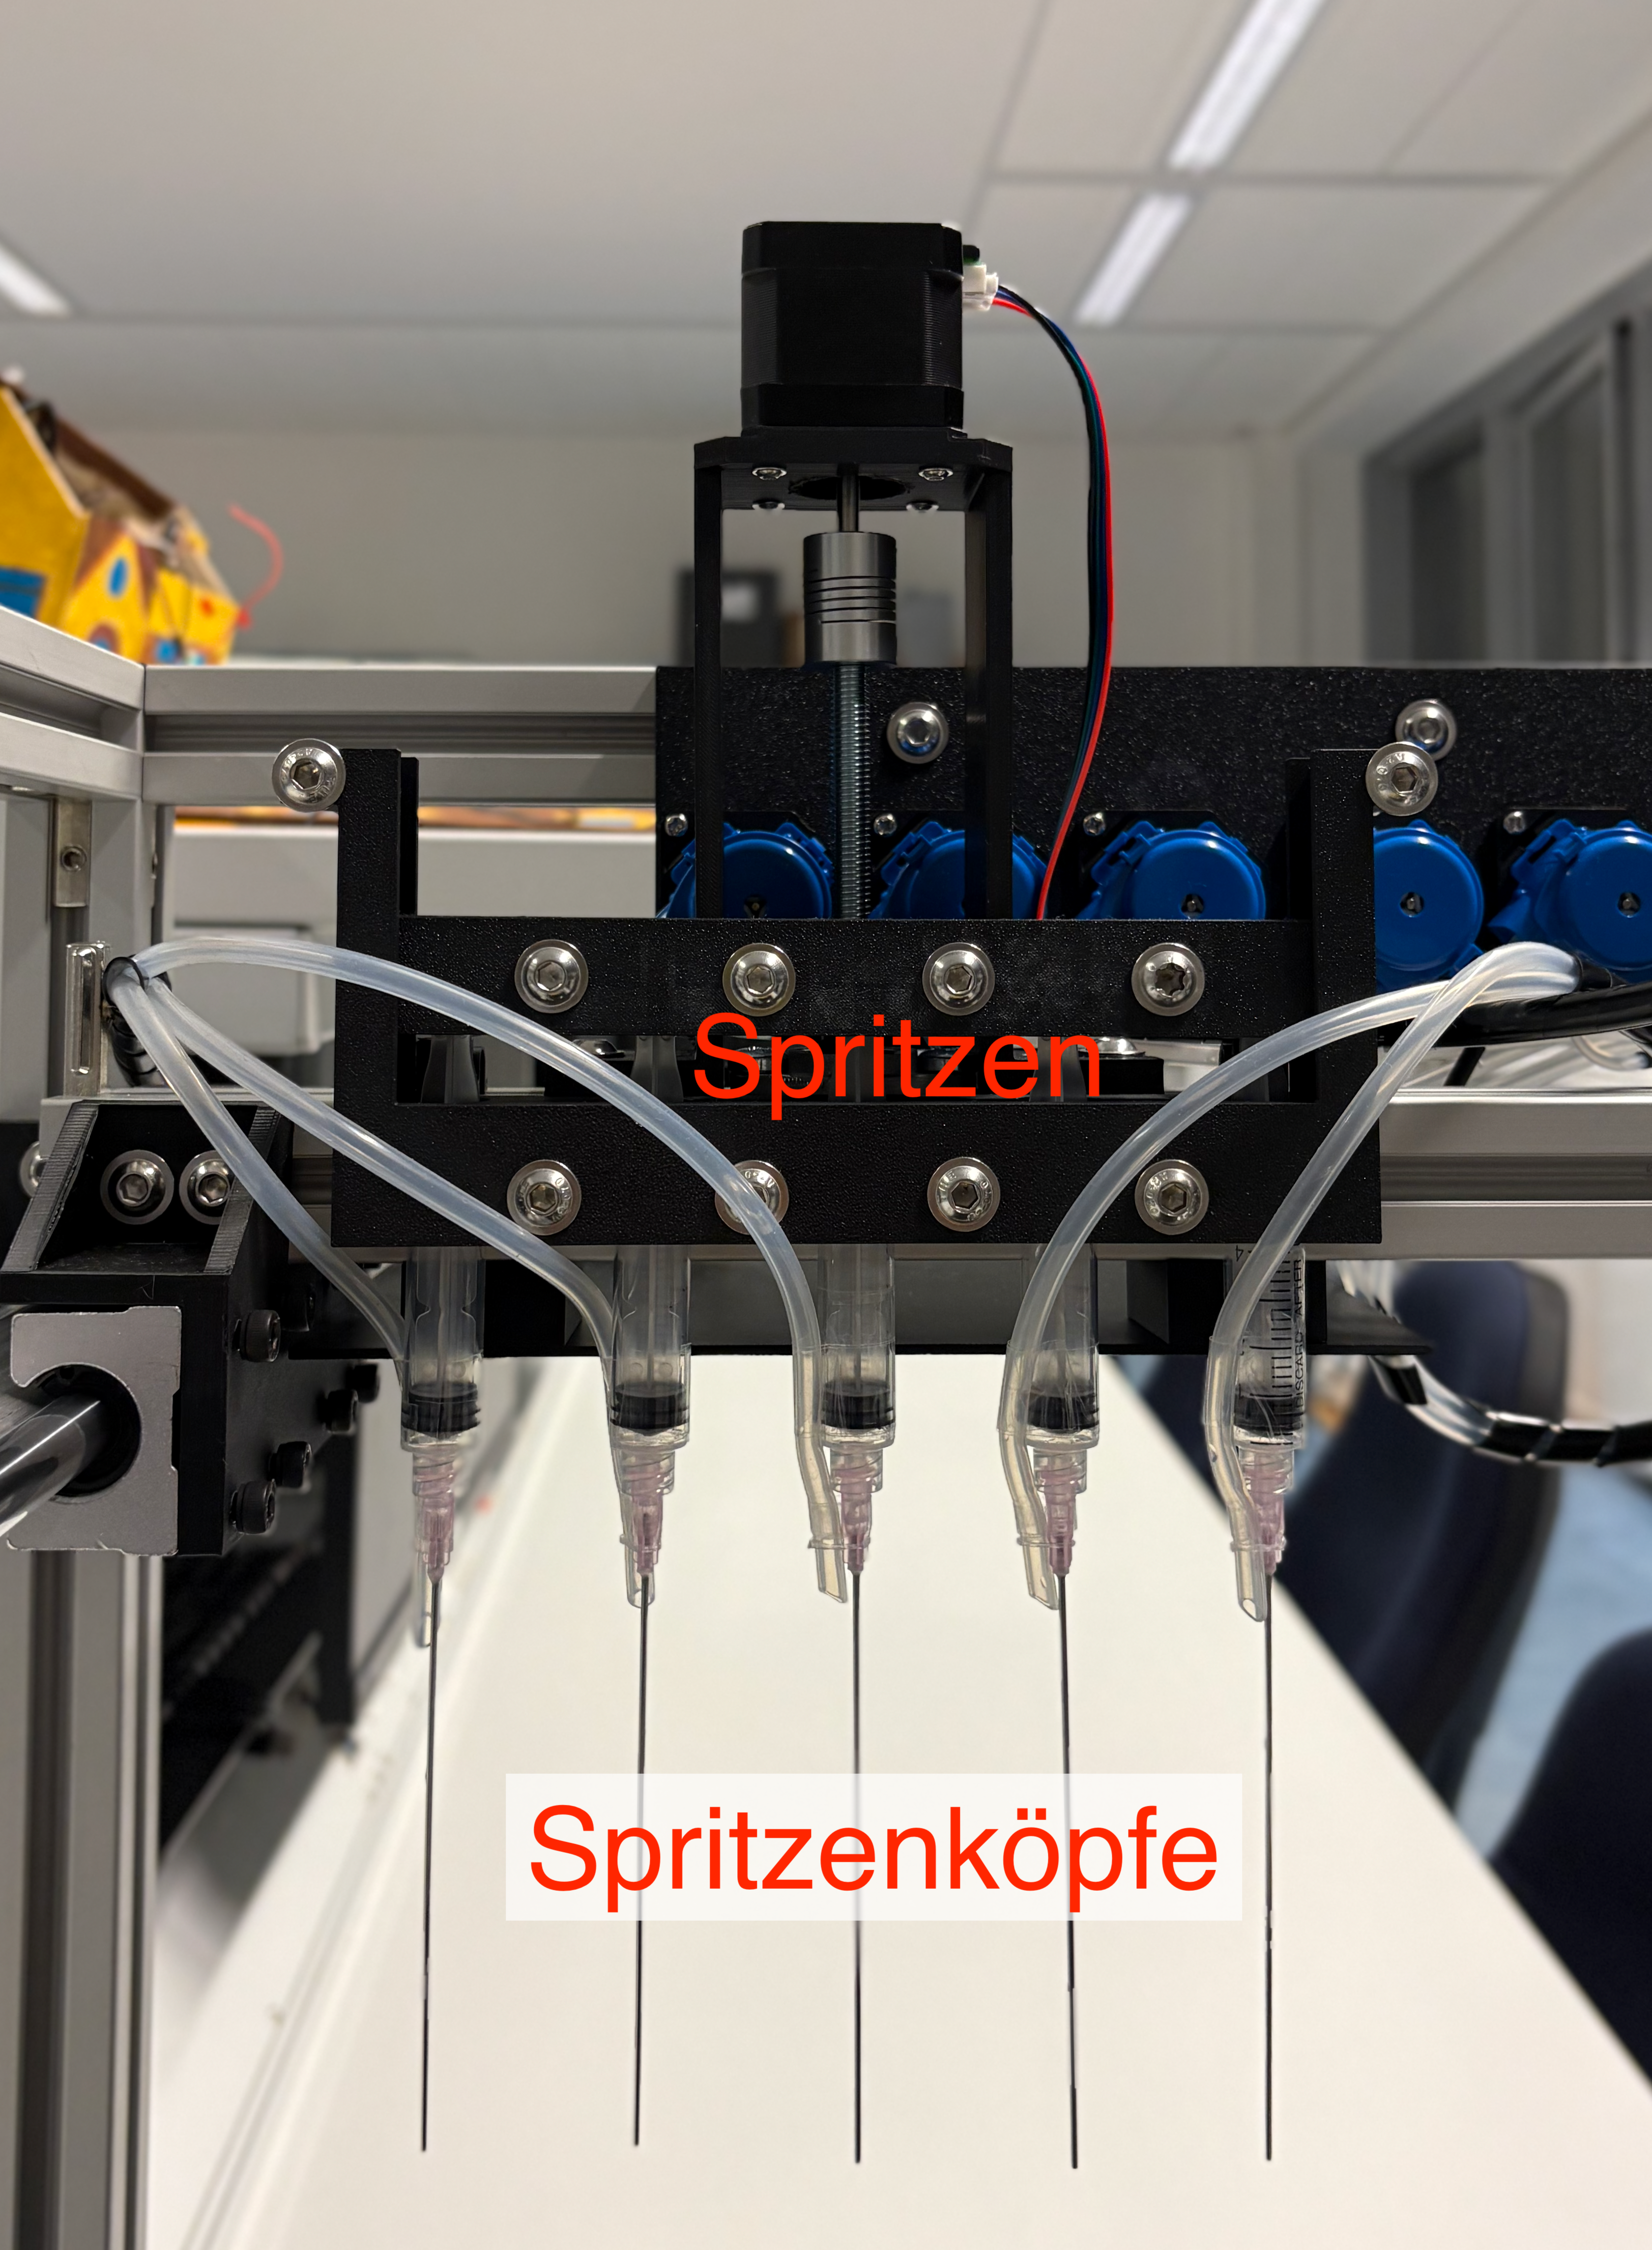
\includegraphics[width=0.7\textwidth]{images/Spritzen.png}
    \caption{Spritzen und Spritzenköpfe des Probenverdünners}
    \label{spritzenkopf}
\end{figure}

\subsubsection{Hubtisch}
Auf dem Hubtisch befinden sich der Falcon-Tube-Ständer, ein Reinigungsbehälter, sowie ein Abfallbehälter. Im Normalfall würde dieser manuell über ein Gewinde betätigt werden. In dem Probenverdünner wird jedoch die Hoch-Runter-Bewegung über ein Stepper-Motor automatisiert und kann verschieden Positionen anfahren. Wie zuvor in \autoref{MechanischeSicherheitshinweise} erwähnt musste eine Expandierseil als Notlösung zur Unterstützung des Motors implementiert werden.  \newline
\begin{figure}[H] % r = rechts, l = links
    \centering
    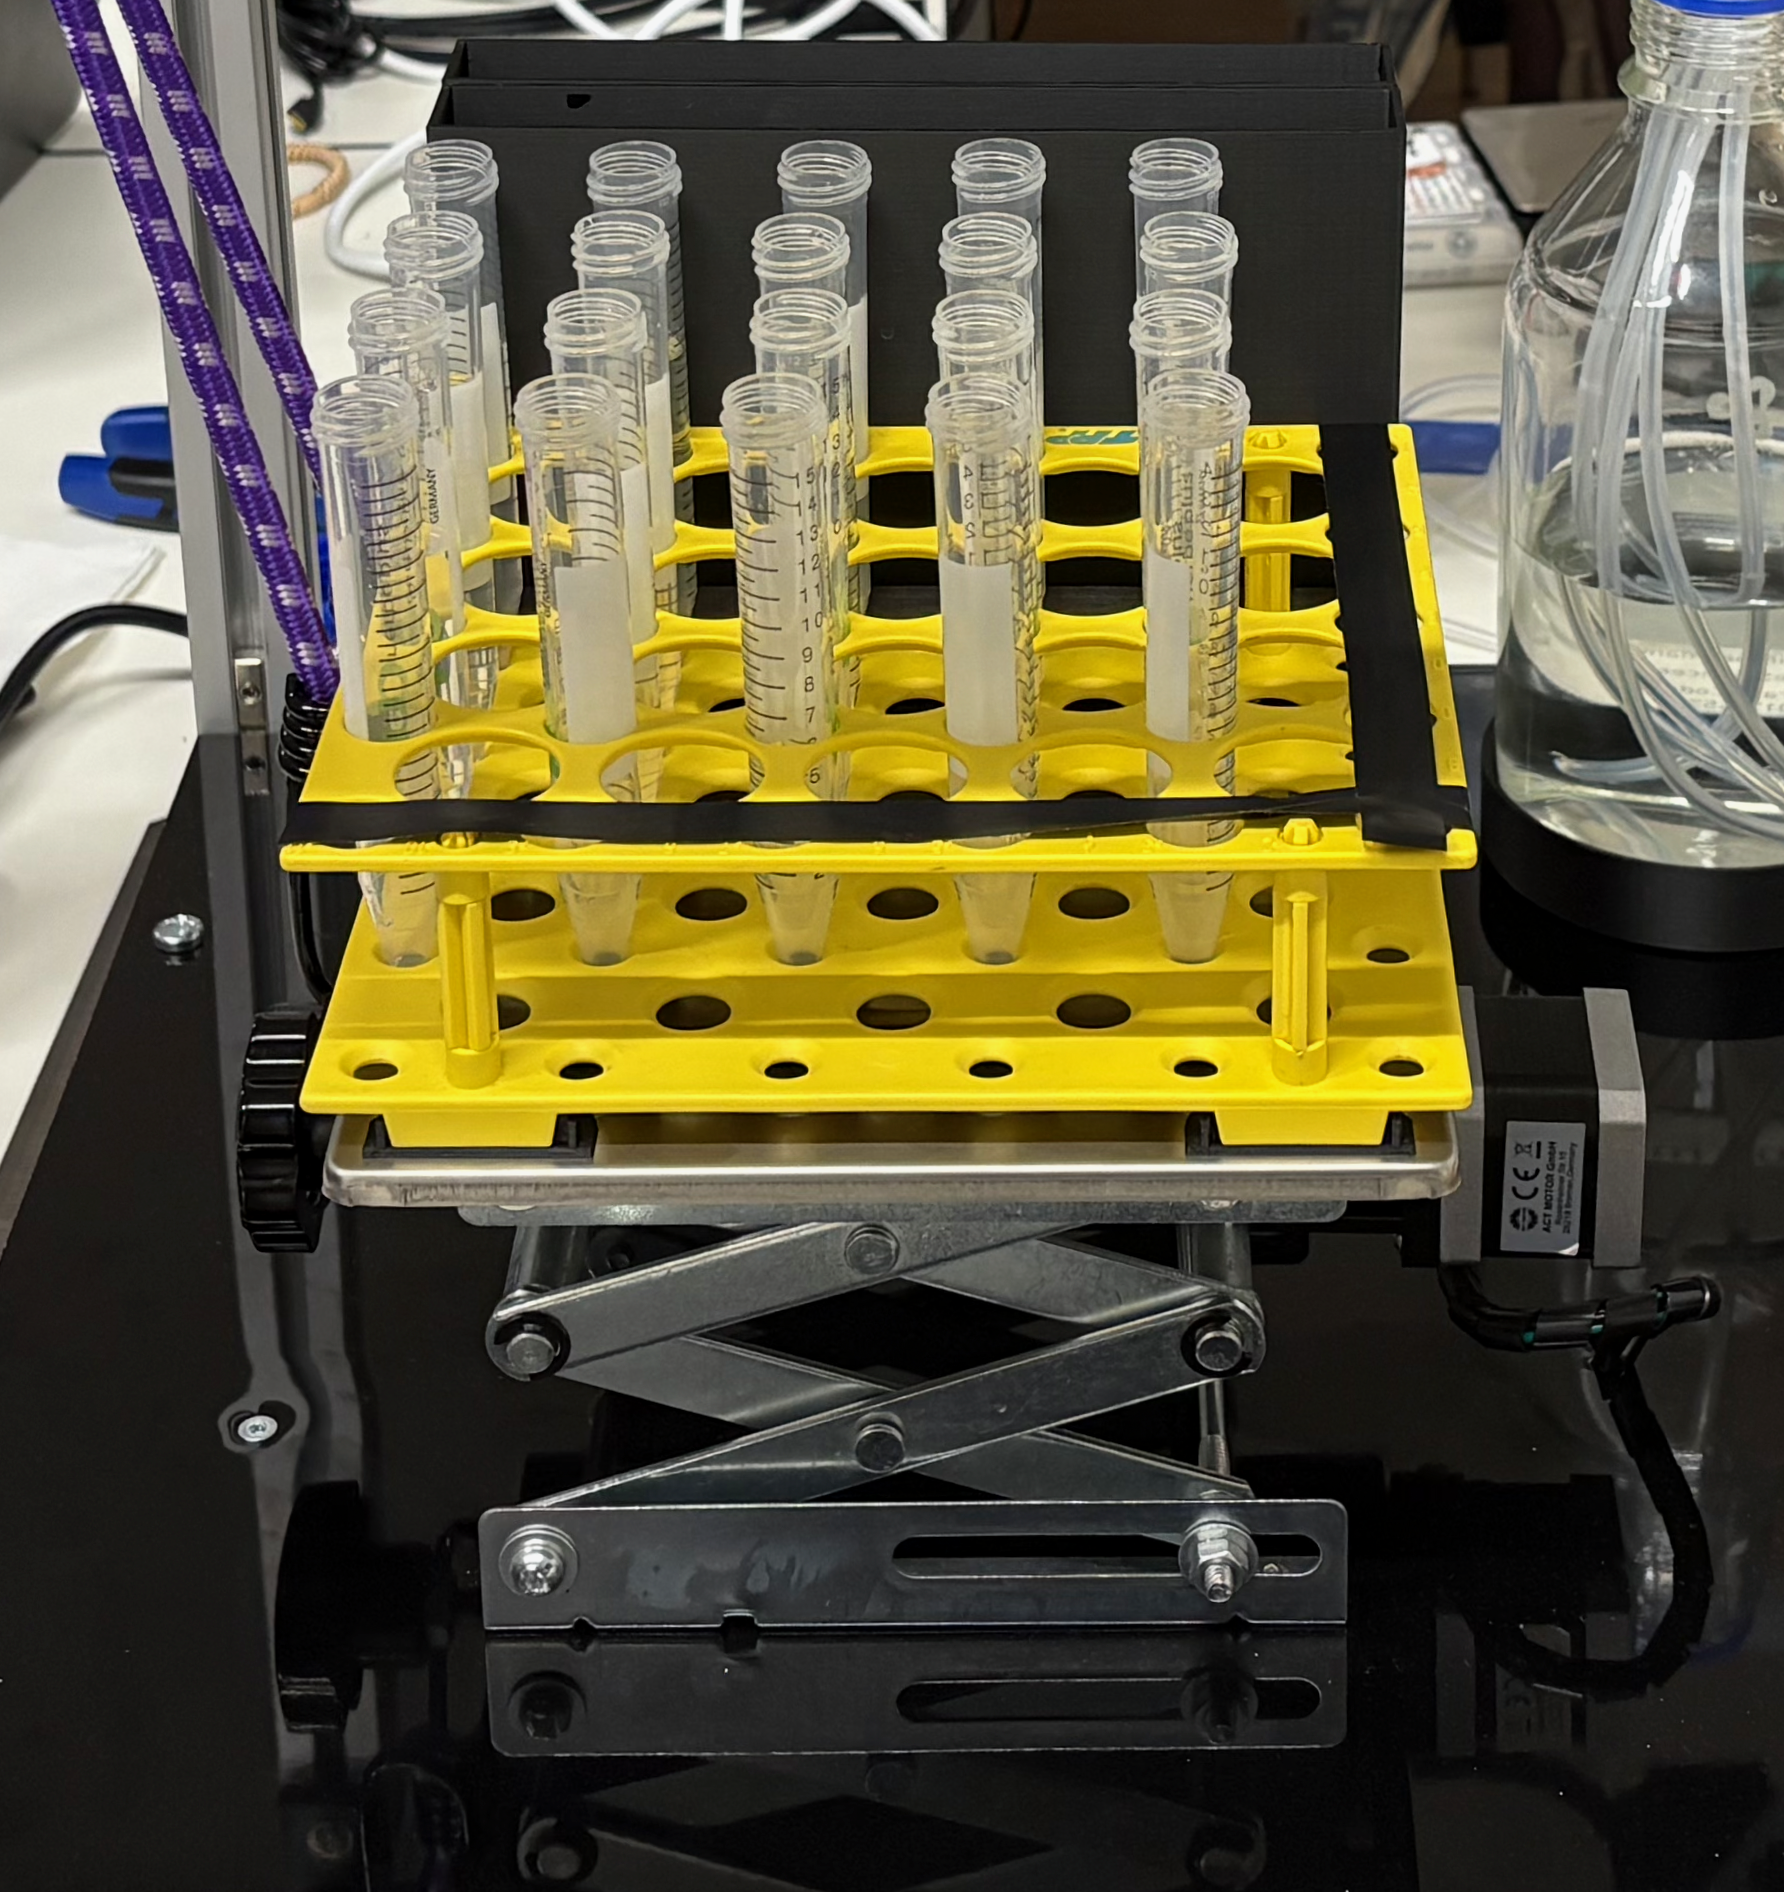
\includegraphics[width=0.7\textwidth]{images/Hubtischvorne.png}
    \caption{Hubtisch des Probenverdünners von vorne}
    \label{Hubtischvorne}
\end{figure}

\subsubsection{Technische Möglichkeiten}\label{TechnischeMoeglichkeiten}
Der Pinkler ist in der Lage 15 Proben in unter 25 Minuten zu befüllen. Der maximale Verdünnungsfaktor beträgt 1/1000. In diesem Fall lassen sich fünf Proben verdünnen. Bei einem Verdünnungsfaktor von unter 1/100 lassen sich zehn verdünnte Proben befüllen und bei einem Verdünnungsfaktor von unter 1/10, 15. Alle Verdünnungsverhältnisse, die nicht vom Probenverdünner umgesetzt werden können, werden durch die Software abgefangen.